\documentclass{article}

%Packages
\usepackage[utf8]{inputenc}
\usepackage{listings}
\usepackage{color}
\usepackage[]{graphicx}
\usepackage{caption}
\usepackage{subcaption}
\usepackage{float}
\usepackage{cleveref}
%\usepackage[bibencoding=utf8]]{biblatex}
\usepackage{indentfirst}
\usepackage[english]{babel}
\usepackage[nottoc]{tocbibind}

%\addbibresource{references.bib}

%% I couldn't do the refernces

\crefformat{figure}{Fig. #1}
\title{2GAQ Molecular Dynamics Simualtion}
\author{Mahmoud Agha}
\date{May 2017}
\graphicspath{{graphs/},{plots/}}
\lstdefinelanguage{mdp}{
morecomment = [l]{;},
morekeywords= {title,define,integrator,nsteps,dt,nstxout,nstvout,nstenergy,nstlog,continuation,constraint_algorithm,constraints,lincs_iter,lincs_order,cutoff-scheme,ns_type,nstlist,rcoulomb,rvdw,coulombtype,pme_order,fourierspacing,tcoupl,tc-grps,tau_t,ref_t,pcoupl,pcoupltype,tau_p,ref_p,compressibility,refcoord_scaling,pbc,DispCorr,gen_vel,include,define,integrator,tinit,dt,nsteps,init-step,simulation-part,comm-mode,nstcomm,comm-grps,bd-fric,ld-seed,emtol,emstep,niter,fcstep,nstcgsteep,nbfgscorr,rtpi,nstxout,nstvout,nstfout,nstlog,nstcalcenergy,nstenergy,nstxout-compressed,compressed-x-precision,compressed-x-grps,energygrps,cutoff-scheme,nstlist,ns_type,pbc,periodic-molecules,verlet-buffer-tolerance,rlist,coulombtype,coulomb-modifier,rcoulomb-switch,rcoulomb,epsilon-r,epsilon-rf,vdw-type,vdw-modifier,rvdw-switch,rvdw,DispCorr,table-extension,energygrp-table,fourierspacing,fourier-nx,fourier-ny,fourier-nz,pme_order,ewald-rtol,ewald-rtol-lj,lj-pme-comb-rule,ewald-geometry,epsilon-surface,implicit-solvent,gb-algorithm,nstgbradii,rgbradii,gb-epsilon-solvent,gb-saltconc,gb-obc-alpha,gb-obc-beta,gb-obc-gamma,gb-dielectric-offset,sa-algorithm,sa-surface-tension,tcoupl,nsttcouple,nh-chain-length,print-nose-hoover-chain-variables,tc-grps,tau_t,ref_t,pcoupl,pcoupltype,nstpcouple,tau_p,compressibility,ref_p,refcoord-scaling,QMMM,QMMM-grps,QMmethod,QMMMscheme,QMbasis,QMcharge,QMmult,SH,CASorbitals,CASelectrons,SAon,SAoff,SAsteps,MMChargeScaleFactor,bOPT,bTS,annealing,annealing-npoints,annealing-time,annealing-temp,gen_vel,gen-temp,gen-seed,constraints,constraint_algorithm,continuation,Shake-SOR,shake-tol,lincs_order,lincs_iter,lincs-warnangle,morse,energygrp-excl,nwall,wall-type,wall-r-linpot,wall-atomtype,wall-density,wall-ewald-zfac,pull,rotation,IMD-group,disre,disre-weighting,disre-mixed,disre-fc,disre-tau,nstdisreout,orire,orire-fc,orire-tau,orire-fitgrp,nstorireout,free-energy,couple-moltype,couple-lambda0,couple-lambda1,couple-intramol,init-lambda,init-lambda-state,delta-lambda,nstdhdl,fep-lambdas,mass-lambdas,coul-lambdas,vdw-lambdas,bonded-lambdas,restraint-lambdas,temperature-lambdas,calc-lambda-neighbors,init-lambda-weights,dhdl-print-energy,sc-alpha,sc-power,sc-r-power,sc-sigma,sc-coul,separate-dhdl-file,dhdl-derivatives,dh_hist_size,dh_hist_spacing,acc-grps,accelerate,freezegrps,freezedim,cos-acceleration,deform,simulated-tempering,simulated-tempering-scaling,sim-temp-low,sim-temp-high,E-x,E-xt,E-y,E-yt,E-z,E-zt,swapcoords,adress,user1-grps,user2-grps,userint1,userint2,userint3,userint4,userreal1,userreal2,userreal3,userreal4,title,integrator,nsteps,dt,nstxout,nstvout,nstenergy,nstlog,nstxout-compressed,,compressed-x-grps,continuation,constraint_algorithm,constraints,lincs_iter,lincs_order,cutoff-scheme,ns_type,nstlist,rcoulomb,rvdw,coulombtype,pme_order,fourierspacing,tcoupl,tc-grps,tau_t,ref_t,pcoupl,pcoupltype,tau_p,ref_p,compressibility,pbc,DispCorr,gen_vel,title,define,integrator,nsteps,dt,nstxout,nstvout,nstenergy,nstlog,continuation,constraint_algorithm,constraints,lincs_iter,lincs_order,cutoff-scheme,ns_type,nstlist,rcoulomb,rvdw,coulombtype,pme_order,fourierspacing,tcoupl,tc-grps,tau_t,ref_t,pcoupl,pbc,DispCorr,gen_vel,gen_temp,gen_seed,integrator,emtol,emstep,nsteps,nstlist,cutoff-scheme,ns_type,coulombtype,rcoulomb,rvdw,pbc,integrator,emtol,emstep,nsteps,nstlist,cutoff-scheme,ns_type,coulombtype,rcoulomb,rvdw,pbc}}

\bibliographystyle{ieeetr}
\begin{document}

\maketitle
\begin{abstract}
    In this project we do a Molecular Dynamics simulation on the protein from Homo-Sapiens rapamycin (mTOR).Rapamycin bindds and inhibits mTOR function by via the interaction with FKBP-rapamycin-binding (FRB) domain. We do a molecular dynamics simualtion to see how the protein undergoes different conformations and how it interacts with its environment. We sat the environment as water and ran through a minimization of energy process. We then ran a PCA analysis to analyze the different dominant vibrational or rotational motions that it undergoes.
\end{abstract}

\section{Introduction}
mTOR ( mammalian Target of Rapamycin or mechanistic target of rapamycin) \cref{fig:shot} which is related to the phosphatidylinositol 3-kinase is very critical in cell growth regulation as it participates in two protein complexes, mTORC1 (rapamycin sensitive), and mTORC2 (rapamycin insensitive). The treatment of rapamycin can lead to growth arrest, down regulation of protein synthesis, and upregulation of mRNA degradation.


The comments in the code are extremely important and should not be ignored if full understanding about the project is needed.
\section{Molecular Dynamics}
We used gromacs version 2016.3 to run the simulation, we prepared a code on bash to facilitate things and to be able to compare results.

\begin{figure}[H]
          \centering
          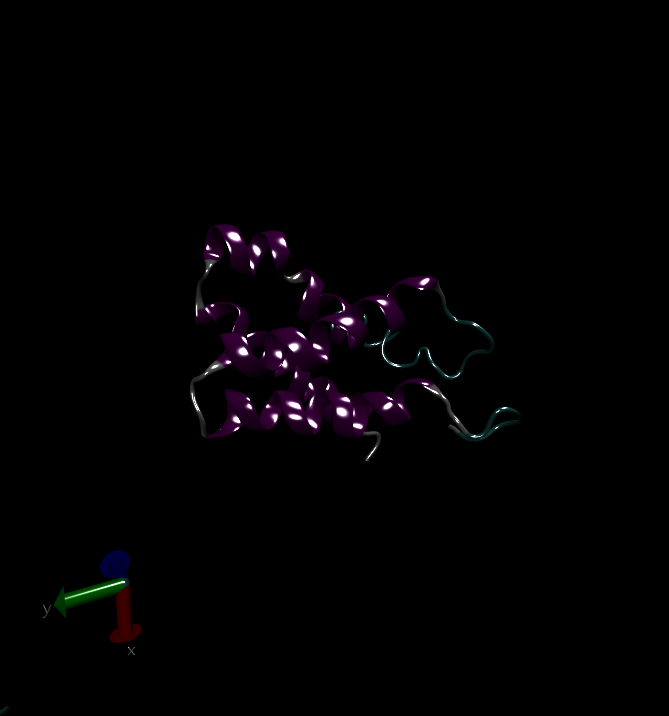
\includegraphics[width=\linewidth]{shot.png}
          \captionof{figure}{The mTOR (2gaq)}
          \label{fig:shot}
\end{figure}

\lstset{commentstyle=\color{blue},stringstyle=\ttfamily,
numbers = left,
numberstyle = \small, frame = single,
breaklines=true,
emphstyle=\textbf
}
\lstinputlisting[language=sh, caption = MD Simulation Code,
emph={gmx, mkdir}
]{MD.sh}


The parameters that are used in the MD are as following \\
Parameters for adding the ions
\lstinputlisting[language = mdp, caption = ions.mdp]{mdp/ions.mdp}
 
 Parameters for Energy Minimization
 \lstinputlisting[language = mdp, caption = minim.mdp]{mdp/minim.mdp}
 
 Parameters for temperature equilibration
 \lstinputlisting[language = mdp, caption = nvt.mdp]{mdp/nvt.mdp}
 
 Parameter for pressure equilibration
 \lstinputlisting[language = mdp, caption = npt.mdp]{mdp/npt.mdp}
 
 Parameters for the production of MD
 \lstinputlisting[language = mdp, caption = md.mdp]{mdp/md.mdp}
 
 \section{Results of MD Simulation}
 After running the code presented above we obtained the graphs that show how the protein was energy-minimized as well as how the simulation went.
 \subsection{Energy Minimization}
 We first need to run energy minimization in order to relax the protein from any difficult conformation that it may have been in \cref{fig:Enrg1}. One thought that one energy minimization process was not enough so we ran another energy minimization to make sure that we overcome any restrained conformation \cref{fig:Enrg2}

 \begin{figure}[H]
    \centering
    \begin{minipage}{.5\textwidth}
          \centering
          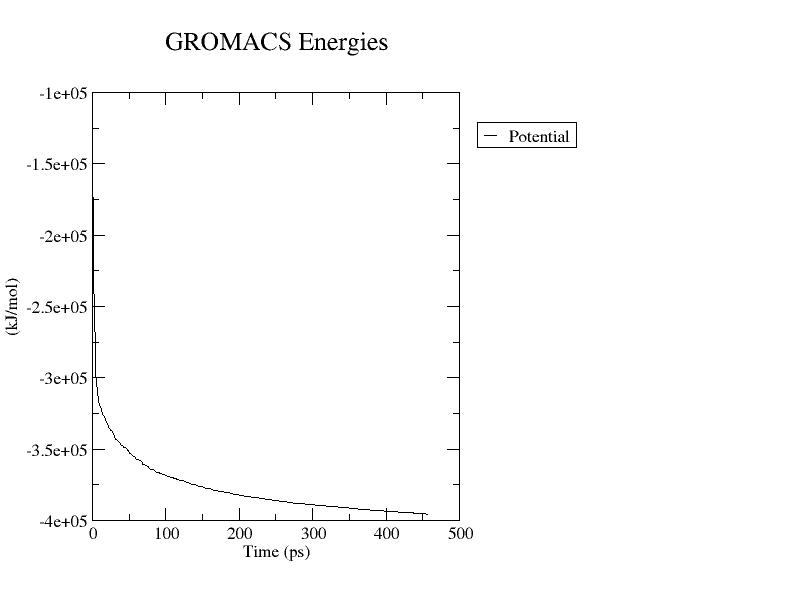
\includegraphics[width=\linewidth]{potential.jpg}
          \captionof{figure}{Energy Minimization I}
          \label{fig:Enrg1}
    \end{minipage}%
    \begin{minipage}{.5\textwidth}
          \centering
          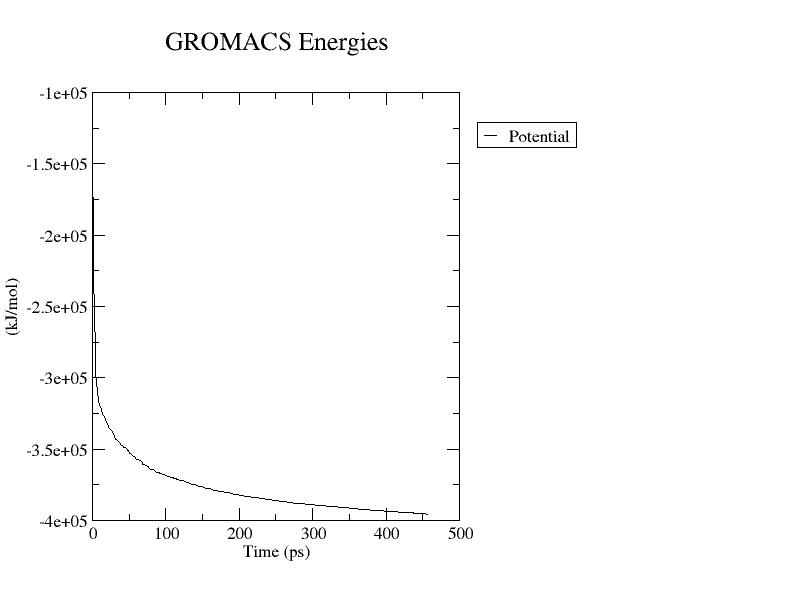
\includegraphics[width=\linewidth]{potential2.jpg}
          \captionof{figure}{Energy Minimization II}
          \label{fig:Enrg2}
    \end{minipage}
\end{figure}

 In order to start MD simulation we need to bring the system (solvent + solute) to equlibrium, we restrained the heavy atoms of the protein to move the solvent without the need to visit any conformation of the protein. Equilibrium is done in two phases with the first one conducted under NVT (constant number of particles, volume and temperature)\footnote{Also referred to as canonical or isothermal-isochoric} \cref{fig:temp}. The second phase is done under NPT (constant number of particles, pressure and temperature)\footnote{Aslo called isothermal-isobaric and is the closest to experimental conditions}. We then analyze the progression of pressure \cref{fig:prs}, and density \cref{fig:dens}
 
  \begin{figure}[H]
     \centering
     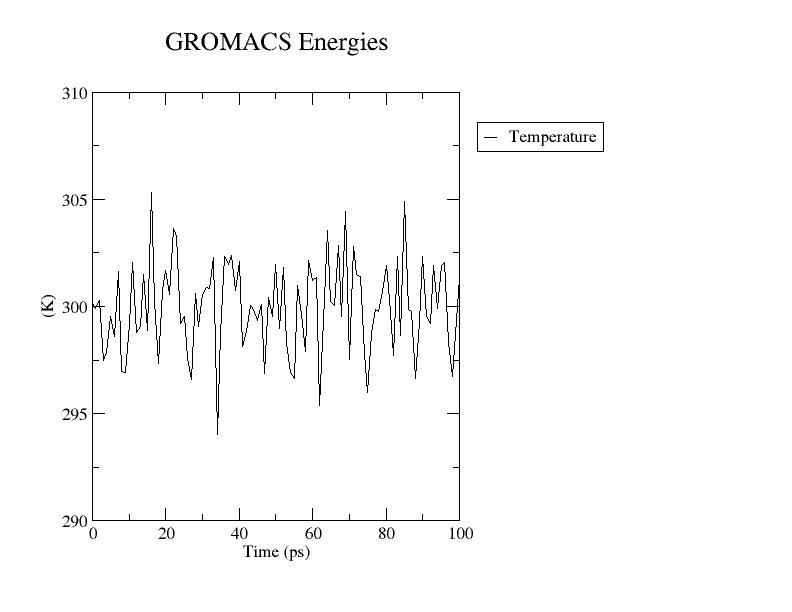
\includegraphics[width= \linewidth]{temperature.jpg}
     \caption{NVT Equilibration}
     \label{fig:temp}
 \end{figure}
 \begin{figure}[H]
    \begin{minipage}{.5\textwidth}
          \centering
          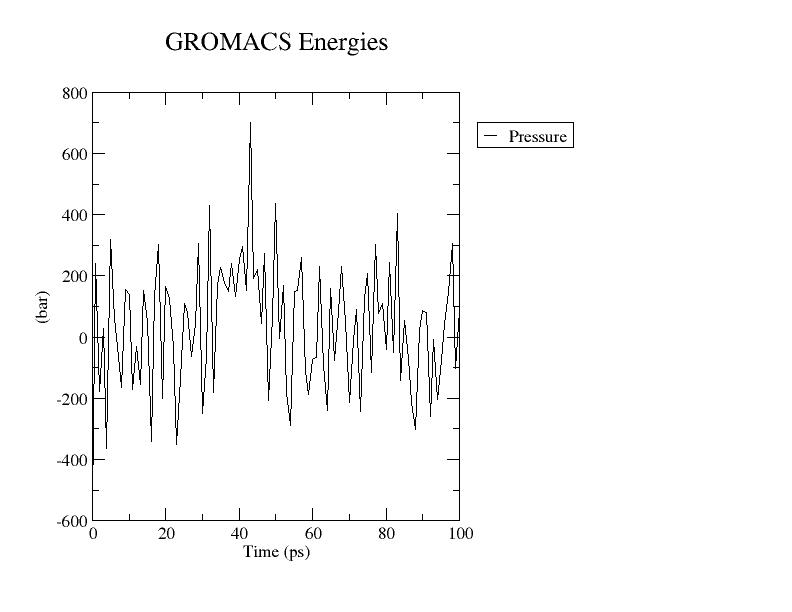
\includegraphics[width=\linewidth]{pressure.jpg}
          \captionof{figure}{NPT Equilibration : Pressure}
          \label{fig:prs}
    \end{minipage}%
    \begin{minipage}{.5\textwidth}
          \centering
          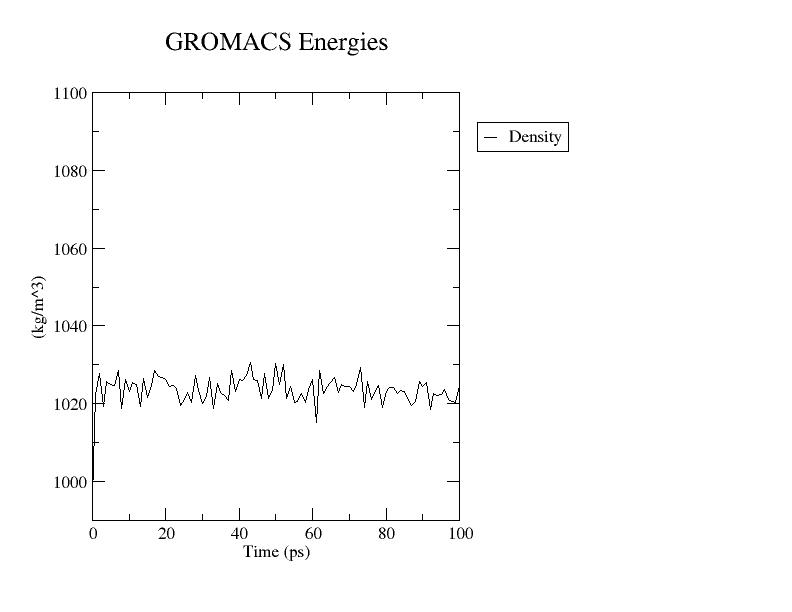
\includegraphics[width=\linewidth]{density.jpg}
          \captionof{figure}{NPT Equilibration : Density}
          \label{fig:dens}
    \end{minipage}
\end{figure}

 
 \section{Analysis of MD Data}
 \label{analMD}
 \subsection{Energy Minimization Process}
 	I noticed that the two energy minimization graphs are identical and I suspect that it has some relation to do with the code. For the second energy minimization instead of using the output of the first energy minimization process I ran another energy minimization process on the old file which would generate the same results. I also did not modify the \emph{mdp} file which could modify the results. The reason I suspect for the slighlty high potential is the difference in electrical charge between solvent and solute as we couldn't equilibrate the two. The charge on the protein was a fraction of the charge of the electron and there was no way (I guess) we could have fixed that.

 \section{Principal Component Analysis}
 \label{pca}
 Before doing a \emph{PCA}\footnote{PCA stands for principal component analysis it shall be called that from now on, it may also be abbreviated to PC which stands for principal component} we needed to transform our trajectory file that was generated by \emph{gromacs} to a file that would be readable by the \emph{R} library \emph{Bio3d}. To do that we used the following code.
 \lstinputlisting[language = python, caption=Transforming from \emph{trj} to \emph{dcd}]{xtcdcd/xtxdcd.py}

 To generate the necessary information and summaries about the \emph{MD} simulation we ran the following \emph{R} code
 \lstinputlisting[language = R, caption = \emph{PCA} and trajectory analysis]{rcode.R}


First we do an \emph{RMSD} analysis on our trajectory \cref{fig:rmsdfrm}, we note that there seems to be no conversion and the protein seems to be over a very large energy barrier, we then do a histogram of the \emph{RMSD} values \cref{fig:rmsdhist} and we notice the absence of a normal distribution curve for our data. This suggests that we did not run the \emph{MD}\footnote{Molecular Dynamics Simulation} for a long enough time or that we are over an energy barrier that we should be crossing and this led us to diverge from the stable conformations that we should have been in. After that we did an \emph{RMSF} analysis \cref{fig:rmsf}. It clearly shows that the termini are the places of high moblity and we need not to worry much about the high values of the \emph{RMSD}

\begin{figure}[H]
          \centering
          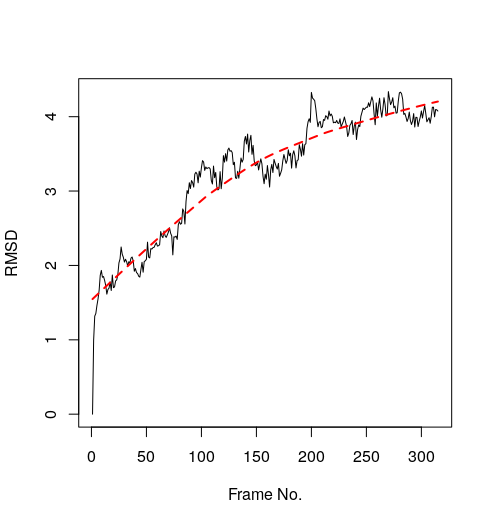
\includegraphics[width=\linewidth]{RMSDvsFrm.png}
          \captionof{figure}{Time series of RMSD which for our case does not show any converstion, it may converge after a few shots though.}
          \label{fig:rmsdfrm}
\end{figure}


  \begin{figure}[H]
          \centering
          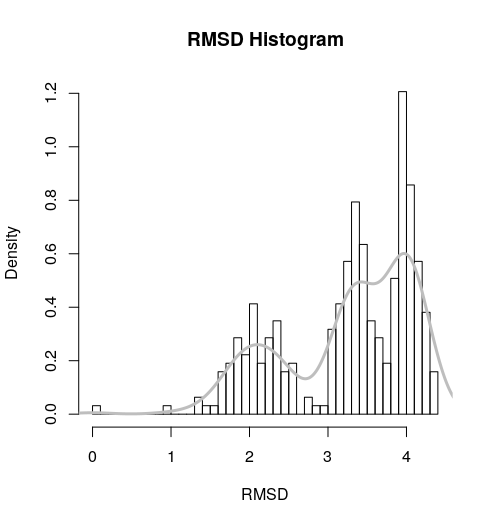
\includegraphics[width=\linewidth]{RMSD.png}
          \captionof{figure}{A histogram to evaluate all the \emph{RMSD} values}
          \label{fig:rmsdhist}
\end{figure}



\begin{figure}[H]
          \centering
          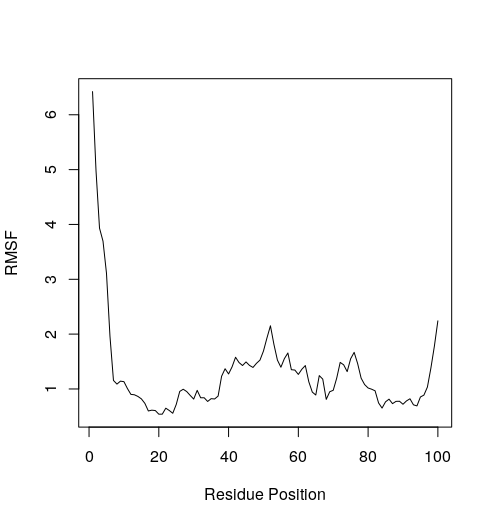
\includegraphics[width=\linewidth]{RMSF.png}
          \captionof{figure}{RMSF with residue number indicates regions of high mobility}
          \label{fig:rmsf}
\end{figure}


Projecting the trajectory on its principal components \cref{fig:pcamul}, we that the protein goes through a distinctive path across time. The mojority of the motion of the protein could be captured by taking the first five principal components more that 82\%, we also note that first principal components comprises about 57.9\% of the motion of the protein. When we do the clustering \cref{fig:pcatwo} we notice the clustering effect very obvious. When we draw the correlation between the residues and the first principal component we note that the termini contribute the most to the motion of the protein. comes second is a region between about resdiue 35 and residue 80. This shows a significant contribution to both the first and the second principal components.

\begin{figure}[H]
          \centering
          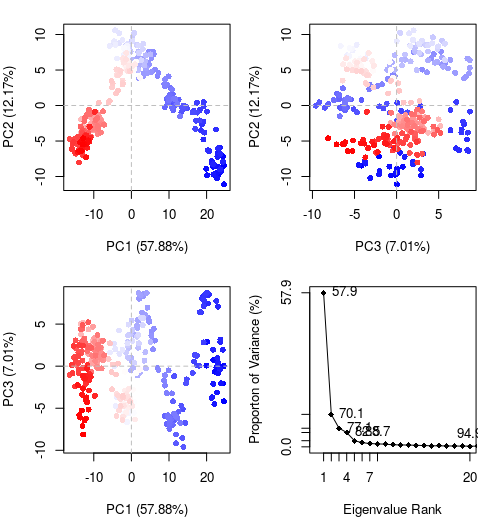
\includegraphics[width=\linewidth]{pcAnalysisMulCol.png}
          \captionof{figure}{PCA for our trajectory that are colored from blue to red in order of time}
          \label{fig:pcamul}
\end{figure}


\begin{figure}[H]
          \centering
          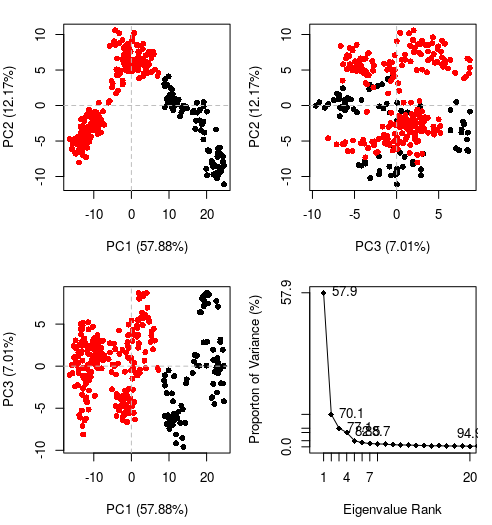
\includegraphics[width=\linewidth]{pcAnalysisTwoCol.png}
          \captionof{figure}{PCA with clustering in PC subspace}
          \label{fig:pcatwo}
\end{figure}


\begin{figure}[H]
          \centering
          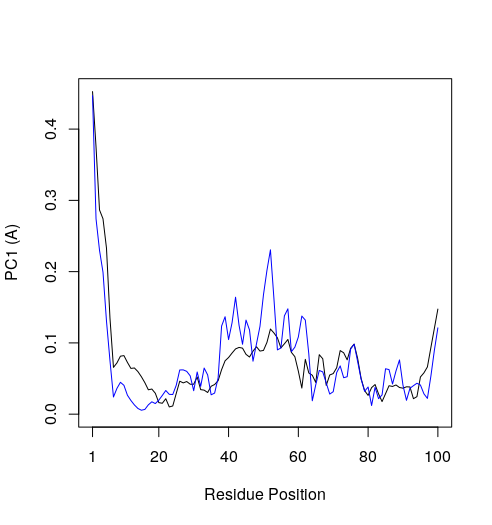
\includegraphics[width=\linewidth]{ResPositionVSpc1.png}
          \captionof{figure}{Contribution of residues to \emph{pc1} and \emph{pc2} the black line is pc1 while the blue is pc2}
          \label{fig:respc}
\end{figure}

The corss correlation between residues \cref{fig:crosscorr} shows that the correlation betwen residues not very high in most regions and does not exceed to maximum correlation, but it falls to negative correlations in a lot of regions.
\begin{figure}[H]
          \centering
          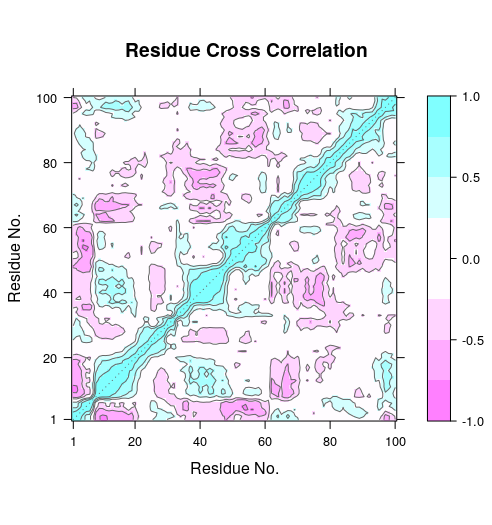
\includegraphics[width=\linewidth]{ResCrossCorr.png}
          \captionof{figure}{Cross Correlation between residues}
          \label{fig:crosscorr}
\end{figure}




 \section{Discussion} % (fold)
 \label{sec:disc}
  The MD simulation was not efficient as it was only run for less than one nanosecond due to lack of hardware resources. We think that if the simulation had enough time to run it would make the results more reliable. The \emph{RMSD} as well as the \emph{RMSF} values show that the termini are very flexible and increase the RMSD value greatly. A suggestion would be to eliminate the values from the termini from the \emph{RMSD} analysis would greatly enhance the results. We chose the force field \emph{OPLS} simply because it worked. We tried other forces as well as other program like \emph{AMBER}, but we couldn't get them to work. They wasted a lot of our time and energy and we should have run the simulation on the force field that we knew produced results anyways. The \emph{PCA} is a little misleading as it captures the movement of the temini which is a little insiginifant in our case.


 \section{Summary}
 \label{sec:sum}
 The protein mTOR (pdb:2gaq) was run in MD simulation with force field \emph{OPLS}. PCA and trajectory analysis were later conducted.
 
 % section section_name (end)


%\bibliography{references}
%\printbibliography
 
\end{document}
